\documentclass{article}

\usepackage{graphicx}

\setlength{\parindent}{4em}
\setlength{\parskip}{1em}

\newcommand{\rt}{$\to\ $}

\begin{document}

    \title{Pre-Read Notes}
    \author{Max C Wong}
    \maketitle

    \section{Chapter 1: Limits and Continuity}

    \subsection{Tangent Lines}
    \begin{itemize}
        \item Limit binds many concepts of Calculus together
        \item With $\frac{\delta y}{\delta x}$, you can approximate slopes
        \item But with curves, it no longer works well
        \item The close you zoom in, say $\rightarrow \infty$ zoom creates a straigh-ish line who's slope can now be approximated
        \item Recall calculating distance between 2 points is $\sqrt{(\delta y)^2 + (\delta x)^2}$
        \item Adding succesive line segments will improve accuracy
    \end{itemize}

    \subsection{Limits}
    \begin{itemize}
        \item Given a function f(x) = L where x gets close to a value a, this would be defined as "L is the limit of f(x) as x appraoches a"
        \item $\lim_{x \to a} f(x)=L$
        \item Restriction at x=a
        \item $\lim_{x \to a} f(x)=L$ Exists if and only if $\lim_{x \to a^-} f(x) = \lim_{x \to a^+} f(x) = L$
    \end{itemize}

    \subsection{Computation of Limits}
    %Insert Diagrams Here (5)

    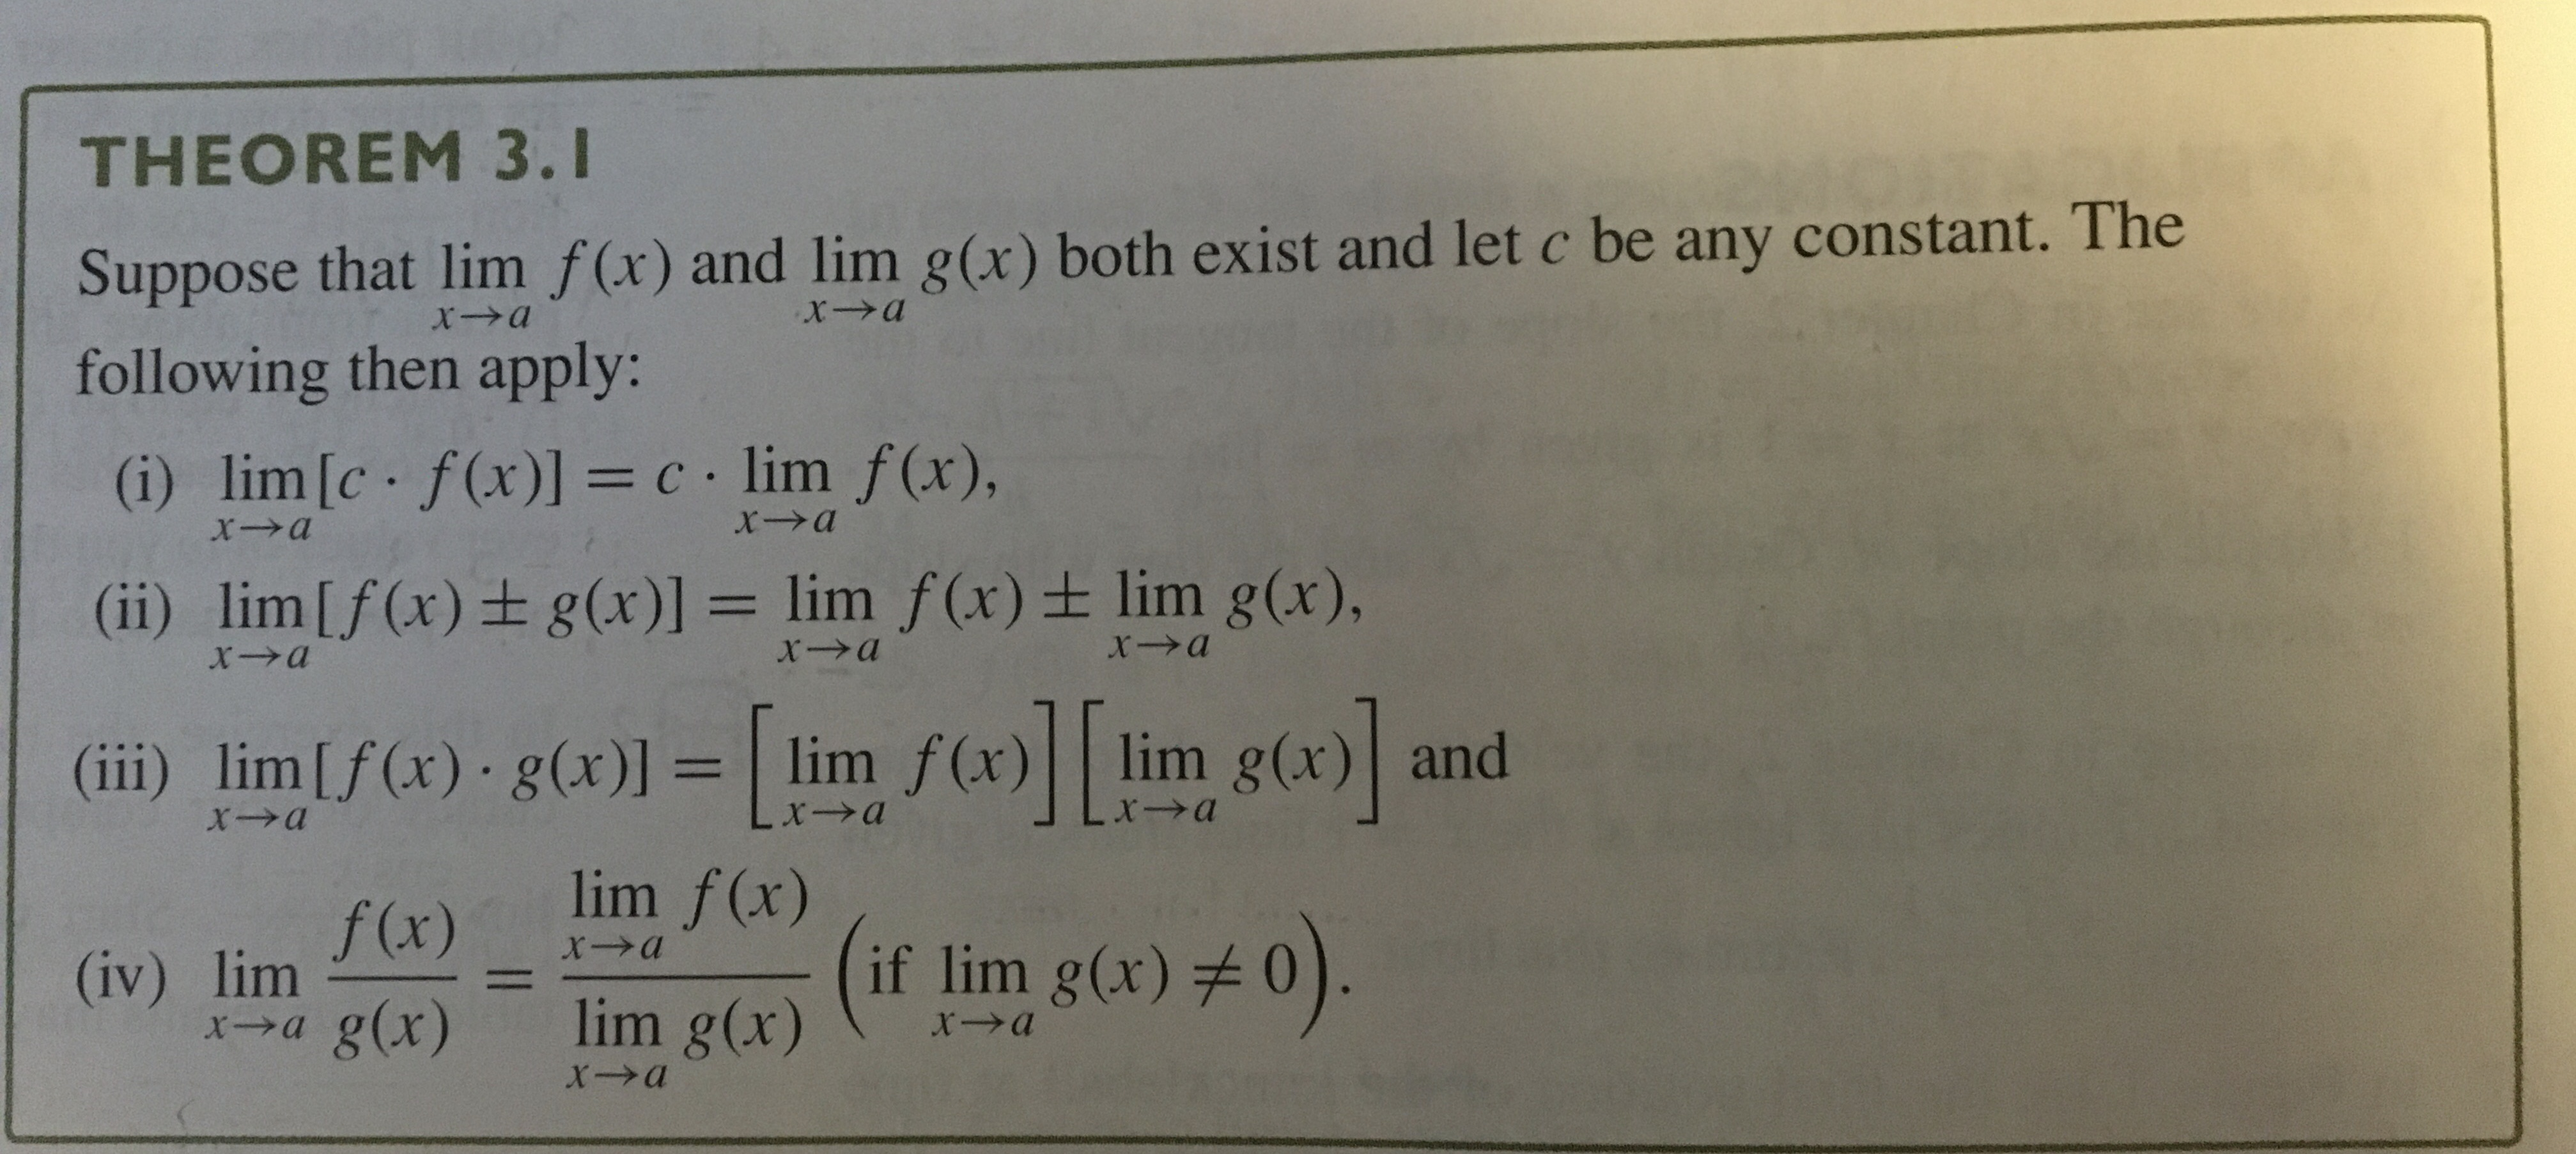
\includegraphics[width=\linewidth]{Pre-Reading/Chapter 1/IMG_0953.JPG}
    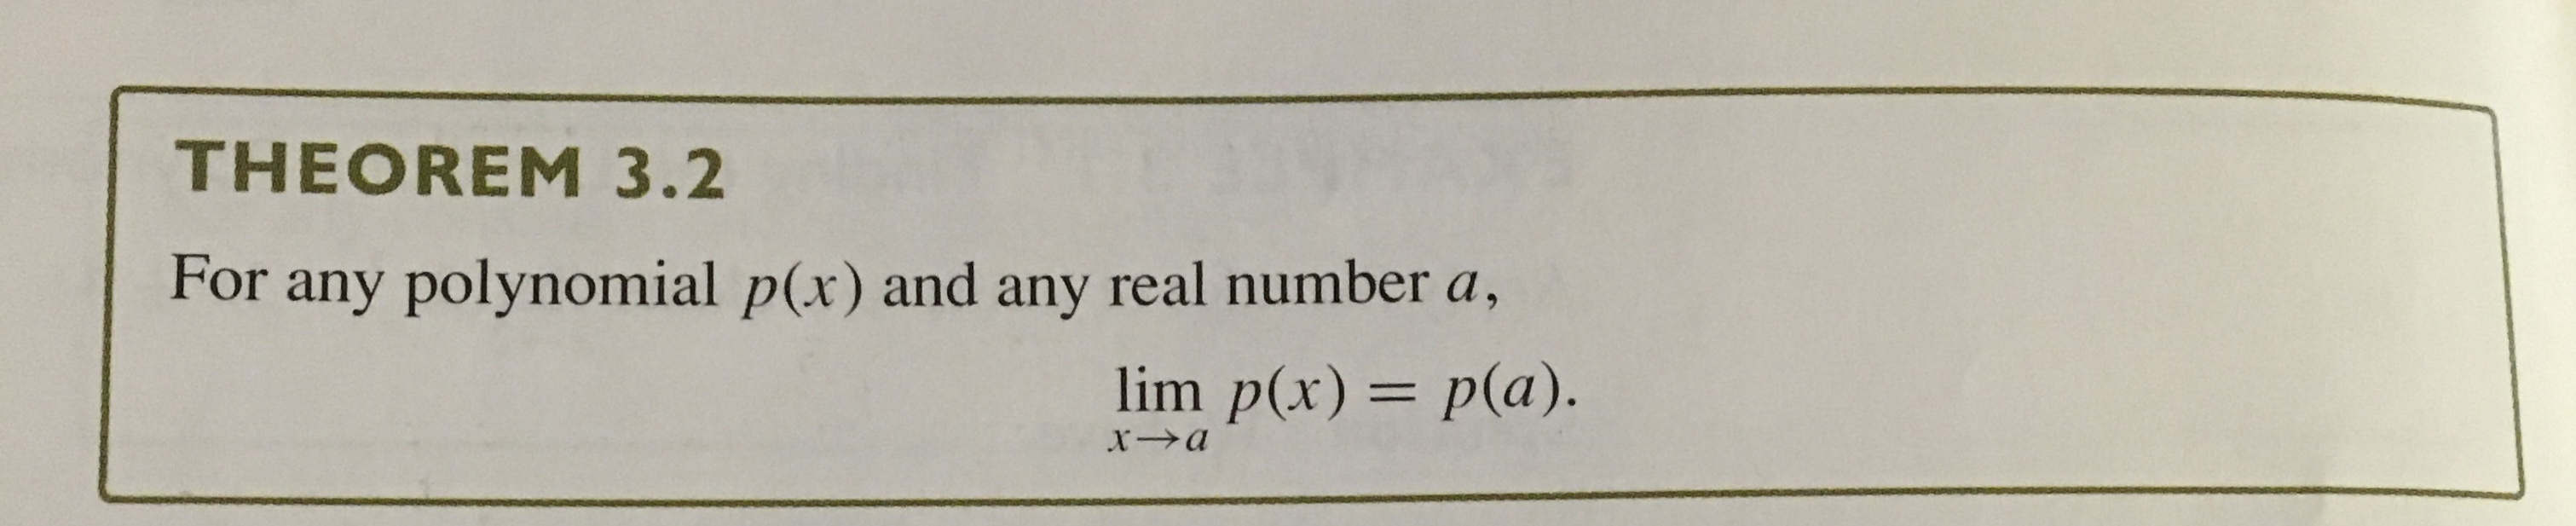
\includegraphics[width=\linewidth]{Pre-Reading/Chapter 1/IMG_0958.JPG}
    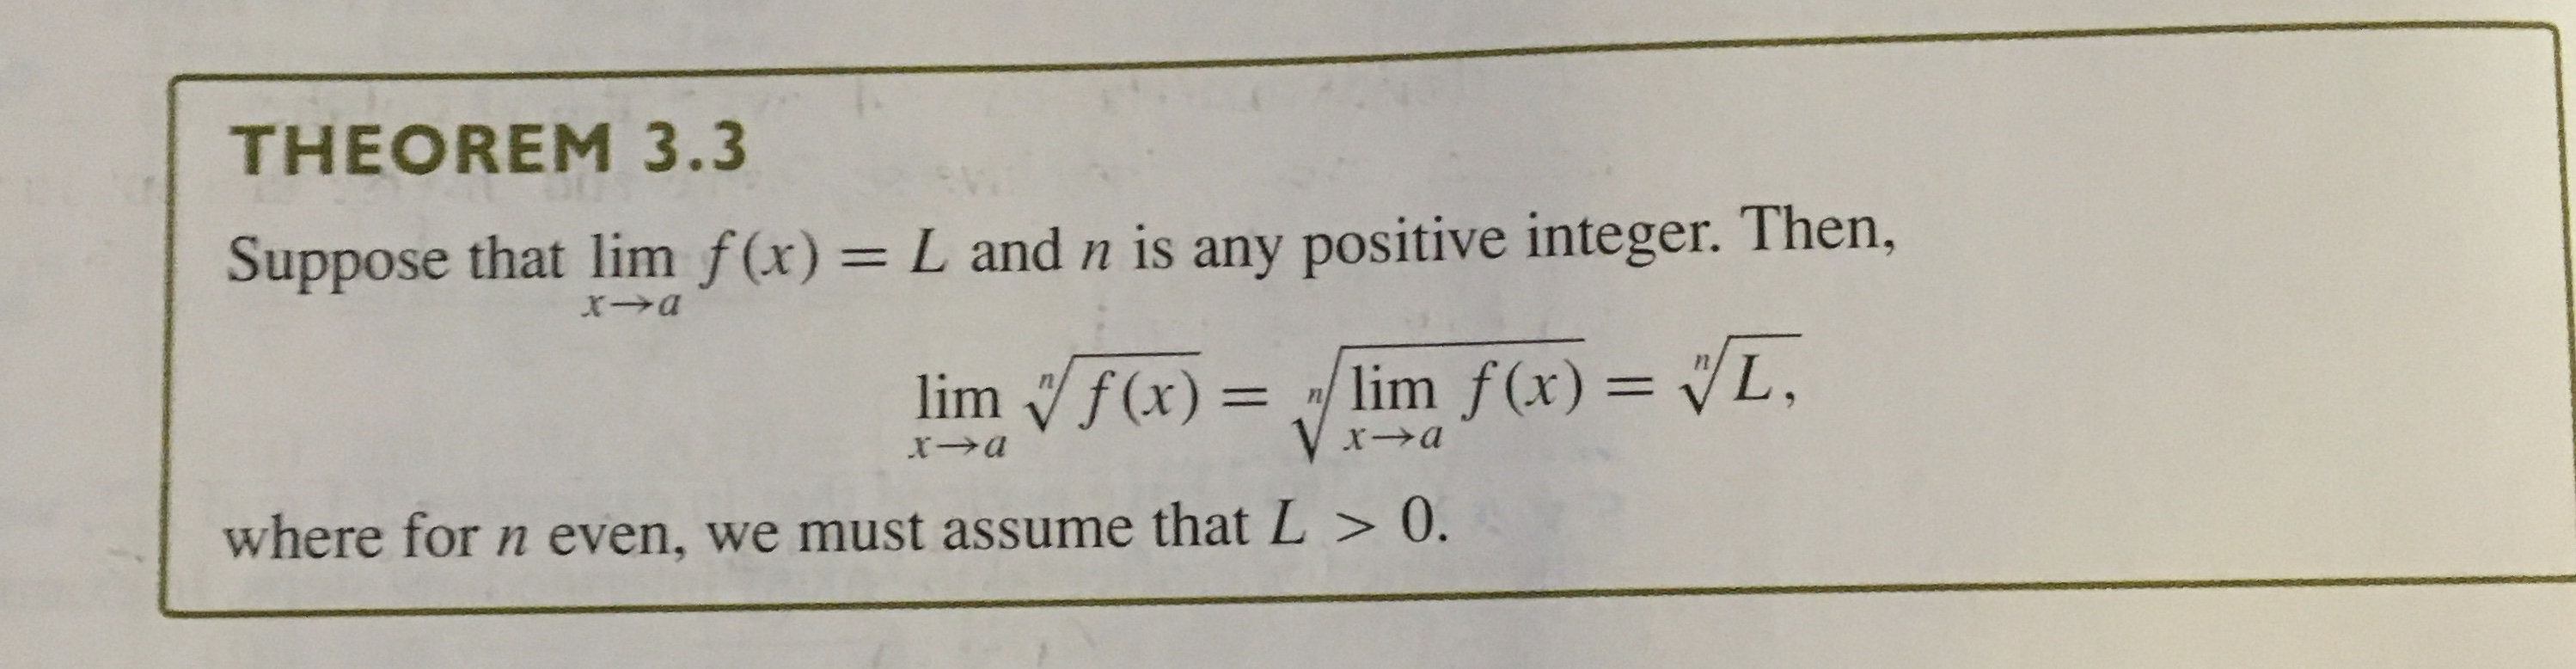
\includegraphics[width=\linewidth]{Pre-Reading/Chapter 1/IMG_0959.JPG}
    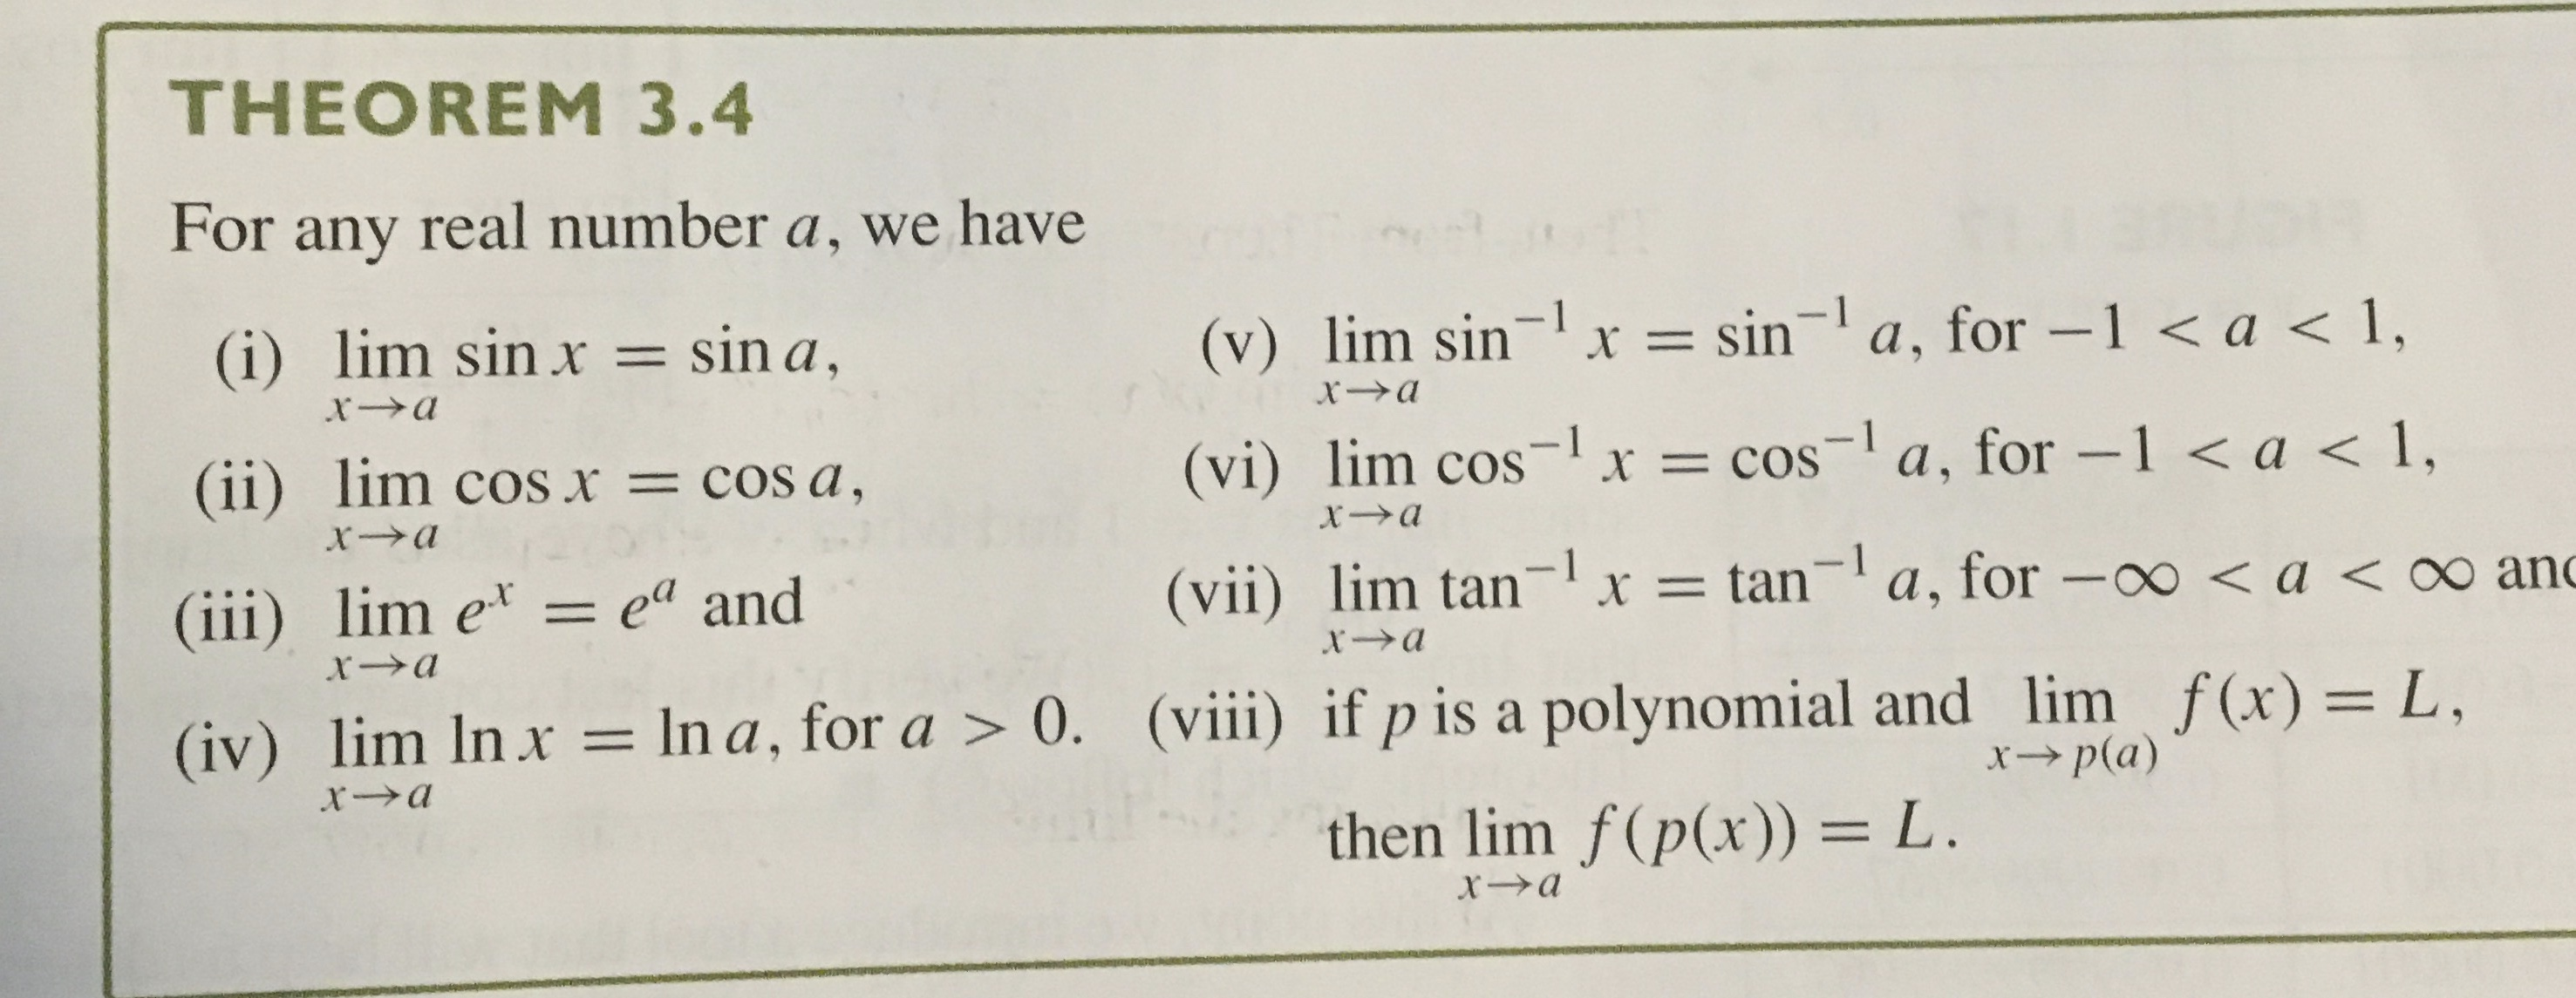
\includegraphics[width=\linewidth]{Pre-Reading/Chapter 1/IMG_0960.JPG}
    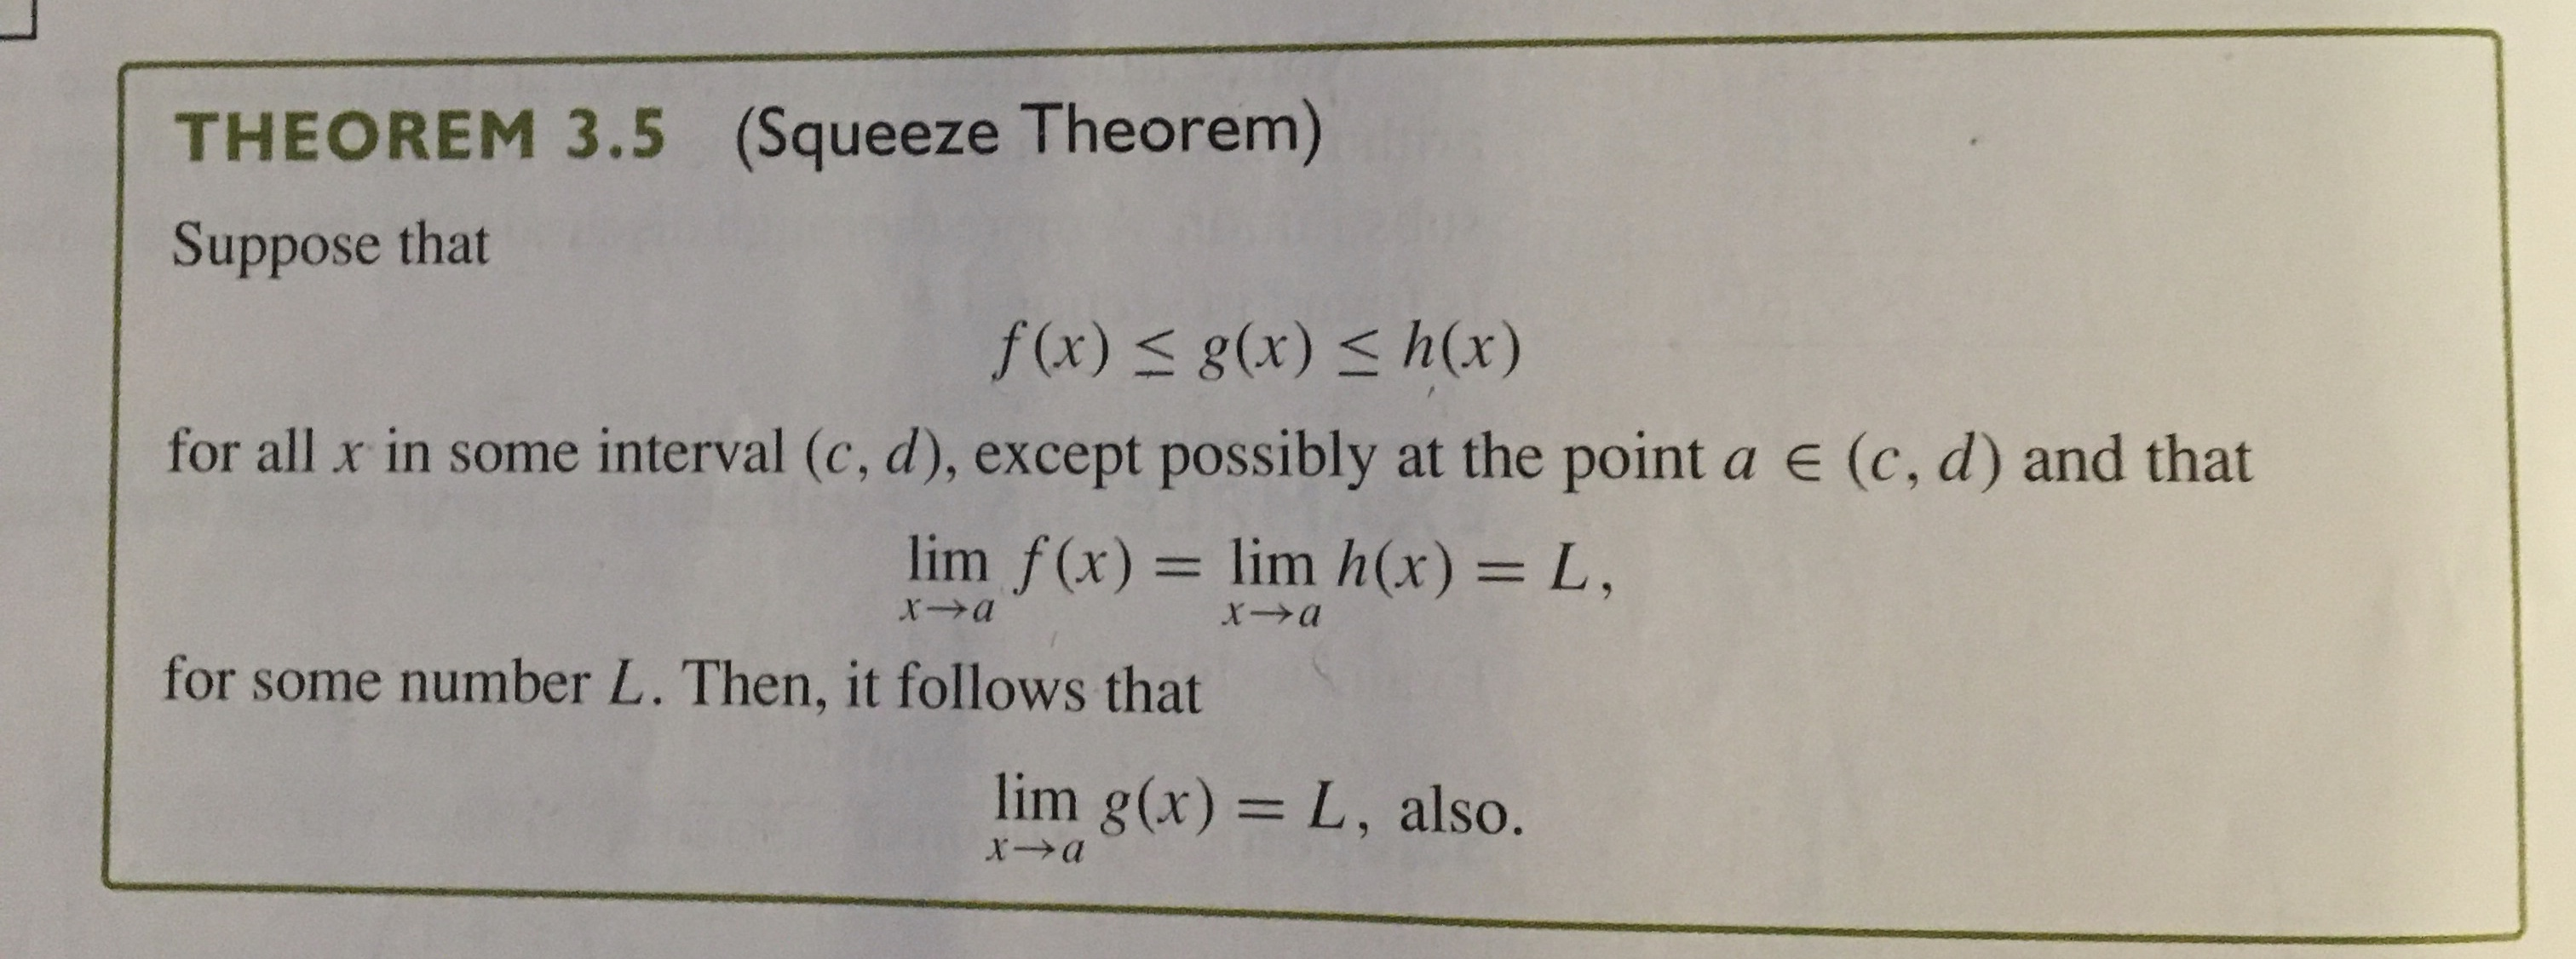
\includegraphics[width=\linewidth]{Pre-Reading/Chapter 1/IMG_0961.JPG}

    \subsection{Continuity and Its Consequences}
    %Insert Diagrams Here (6)

    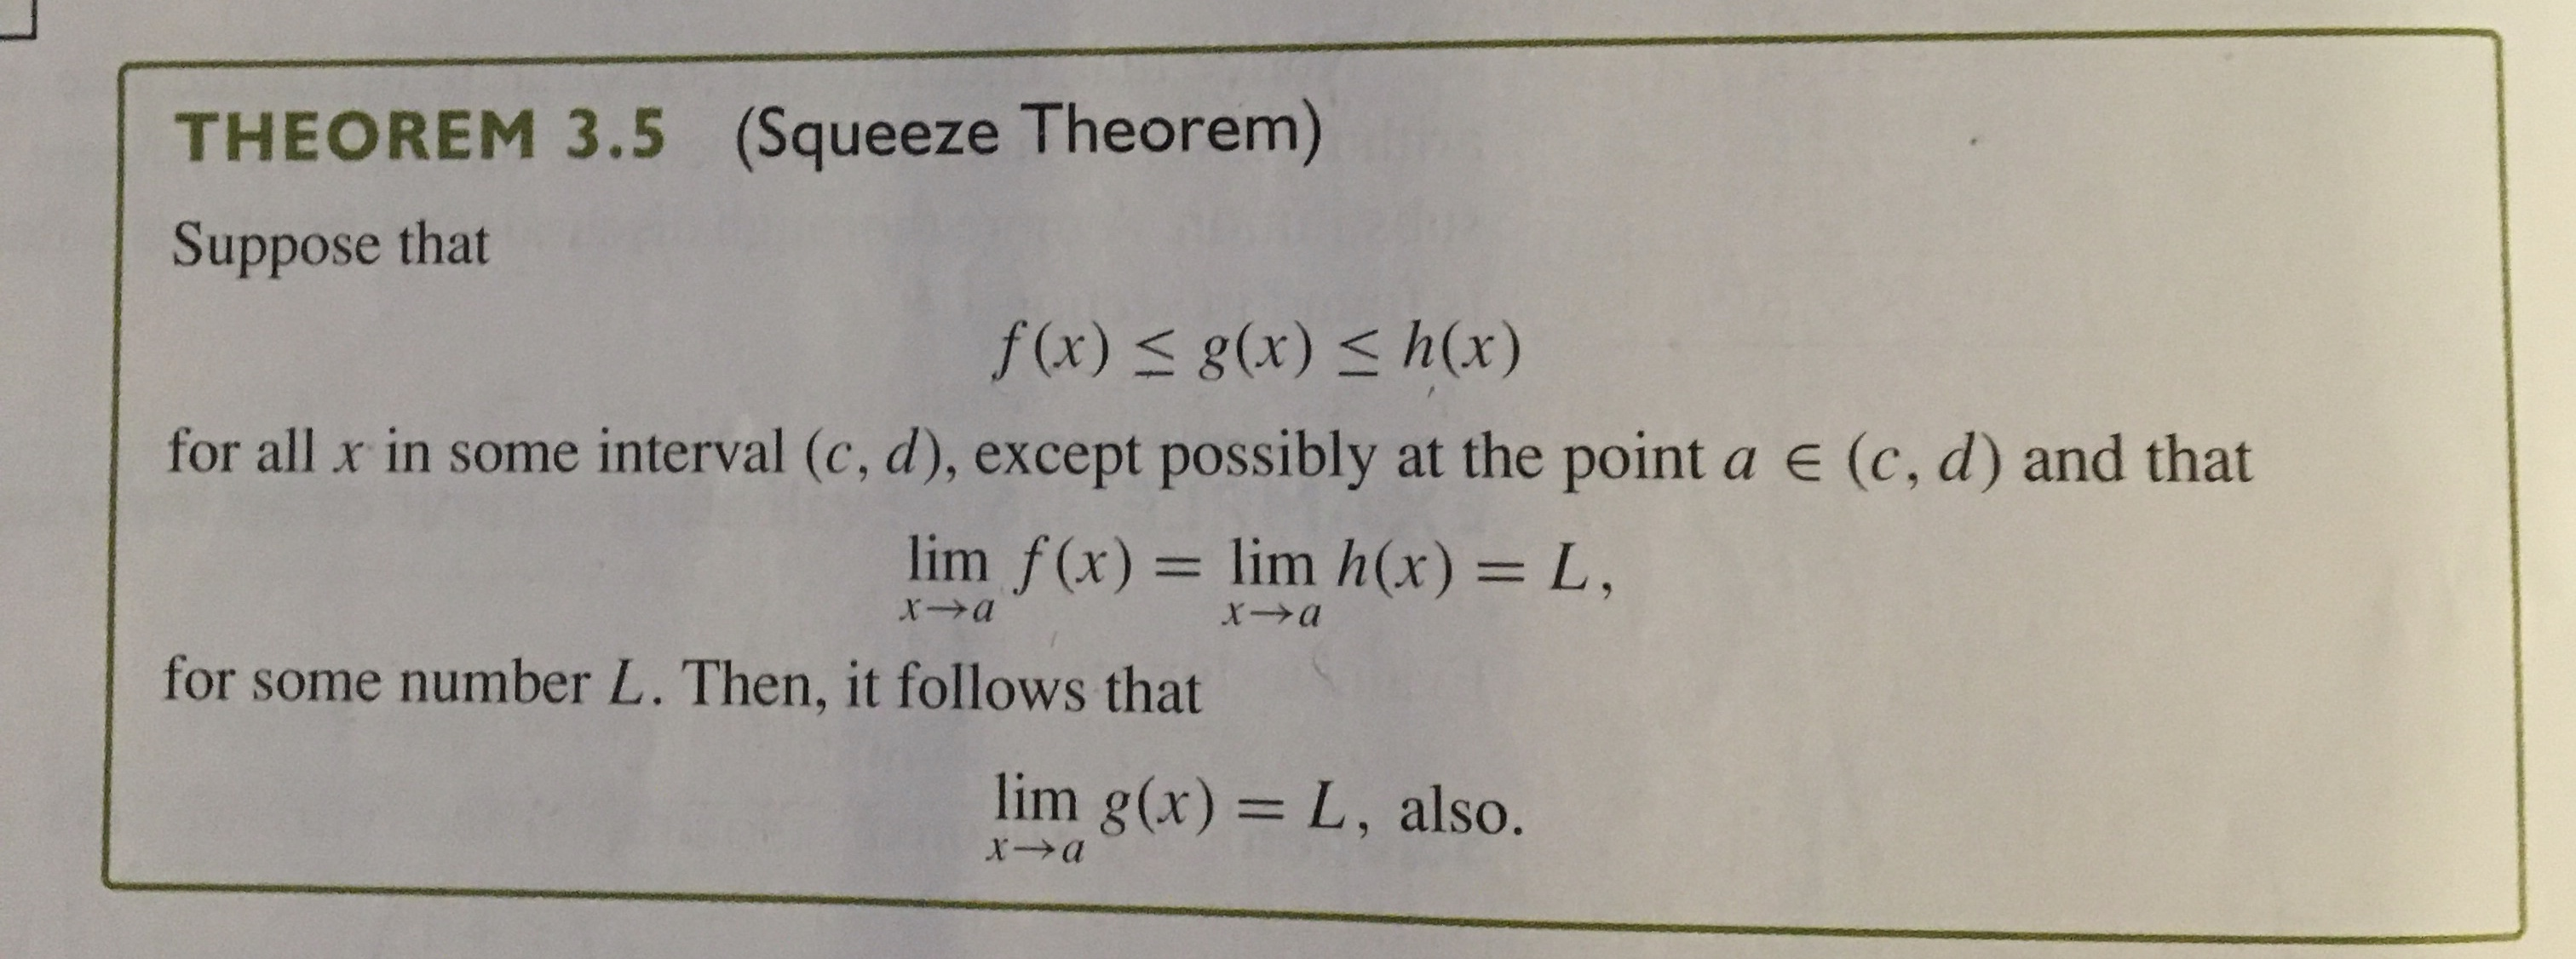
\includegraphics[width=\linewidth]{Pre-Reading/Chapter 1/IMG_0961.JPG}
    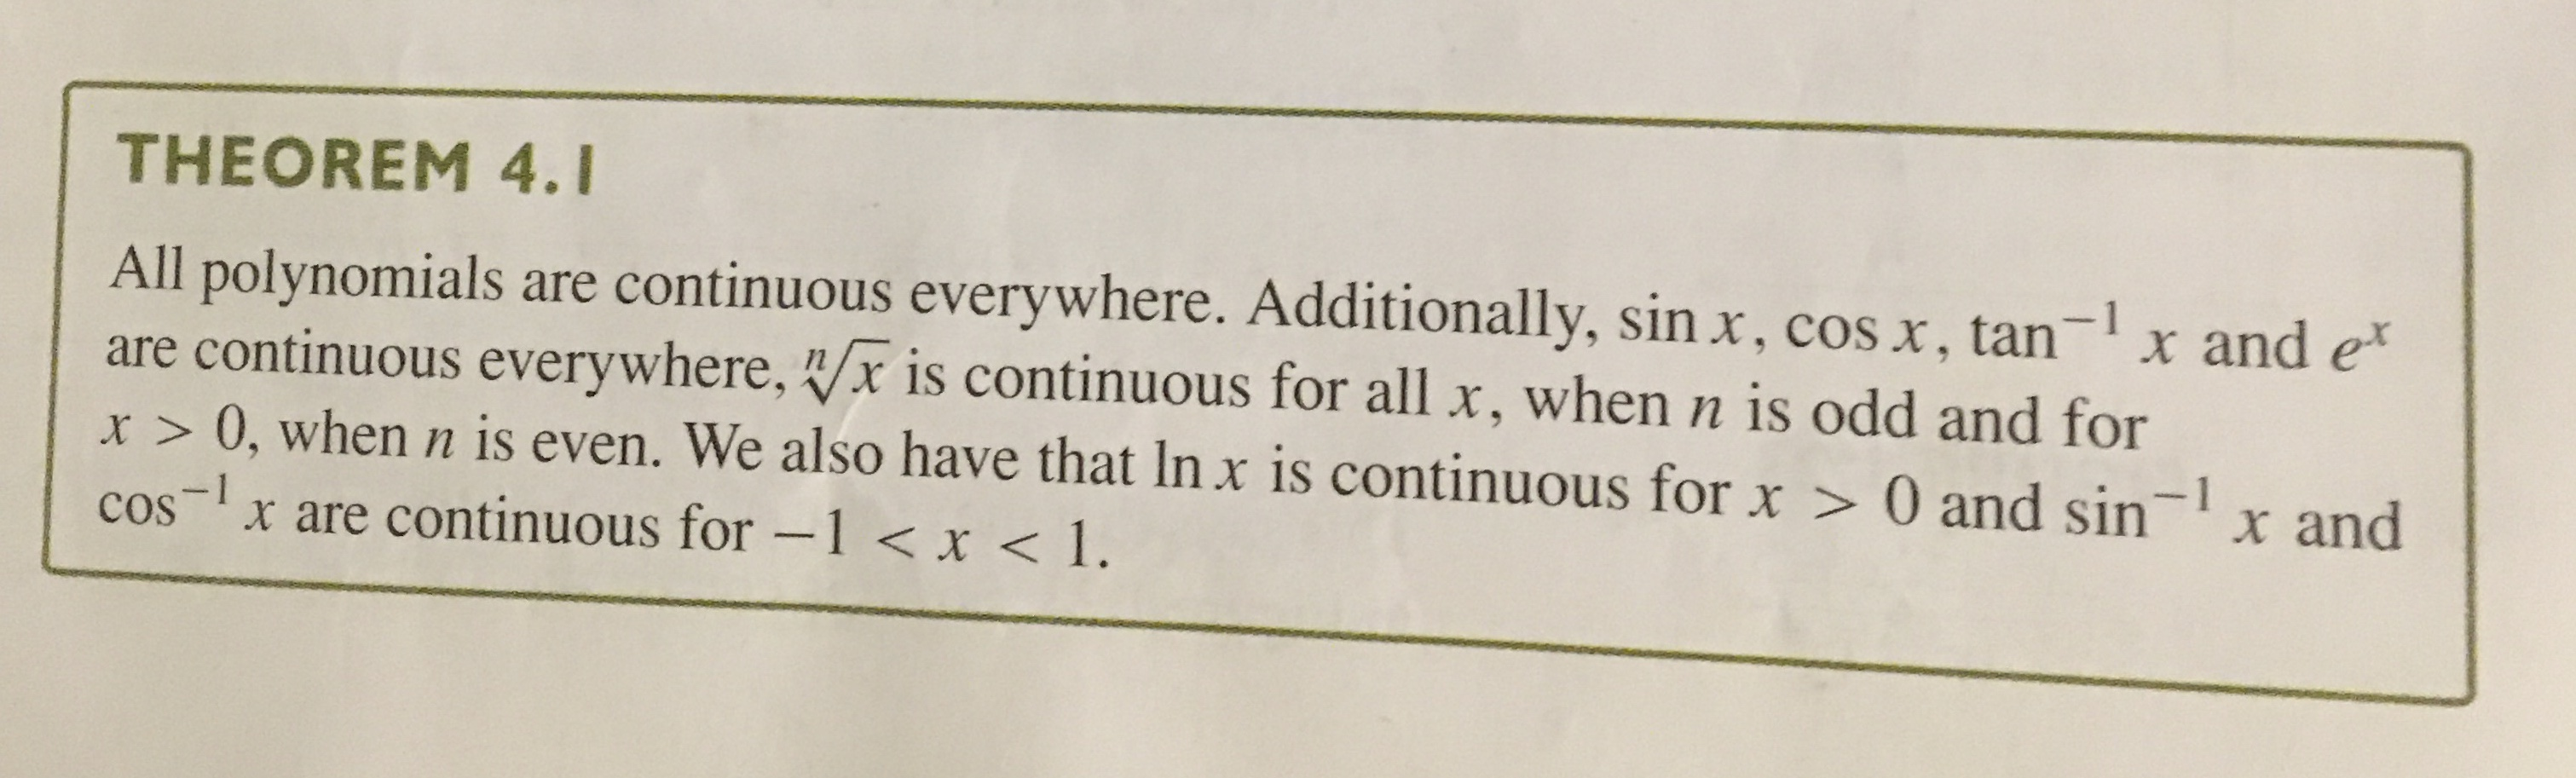
\includegraphics[width=\linewidth]{Pre-Reading/Chapter 1/IMG_0965.JPG}
    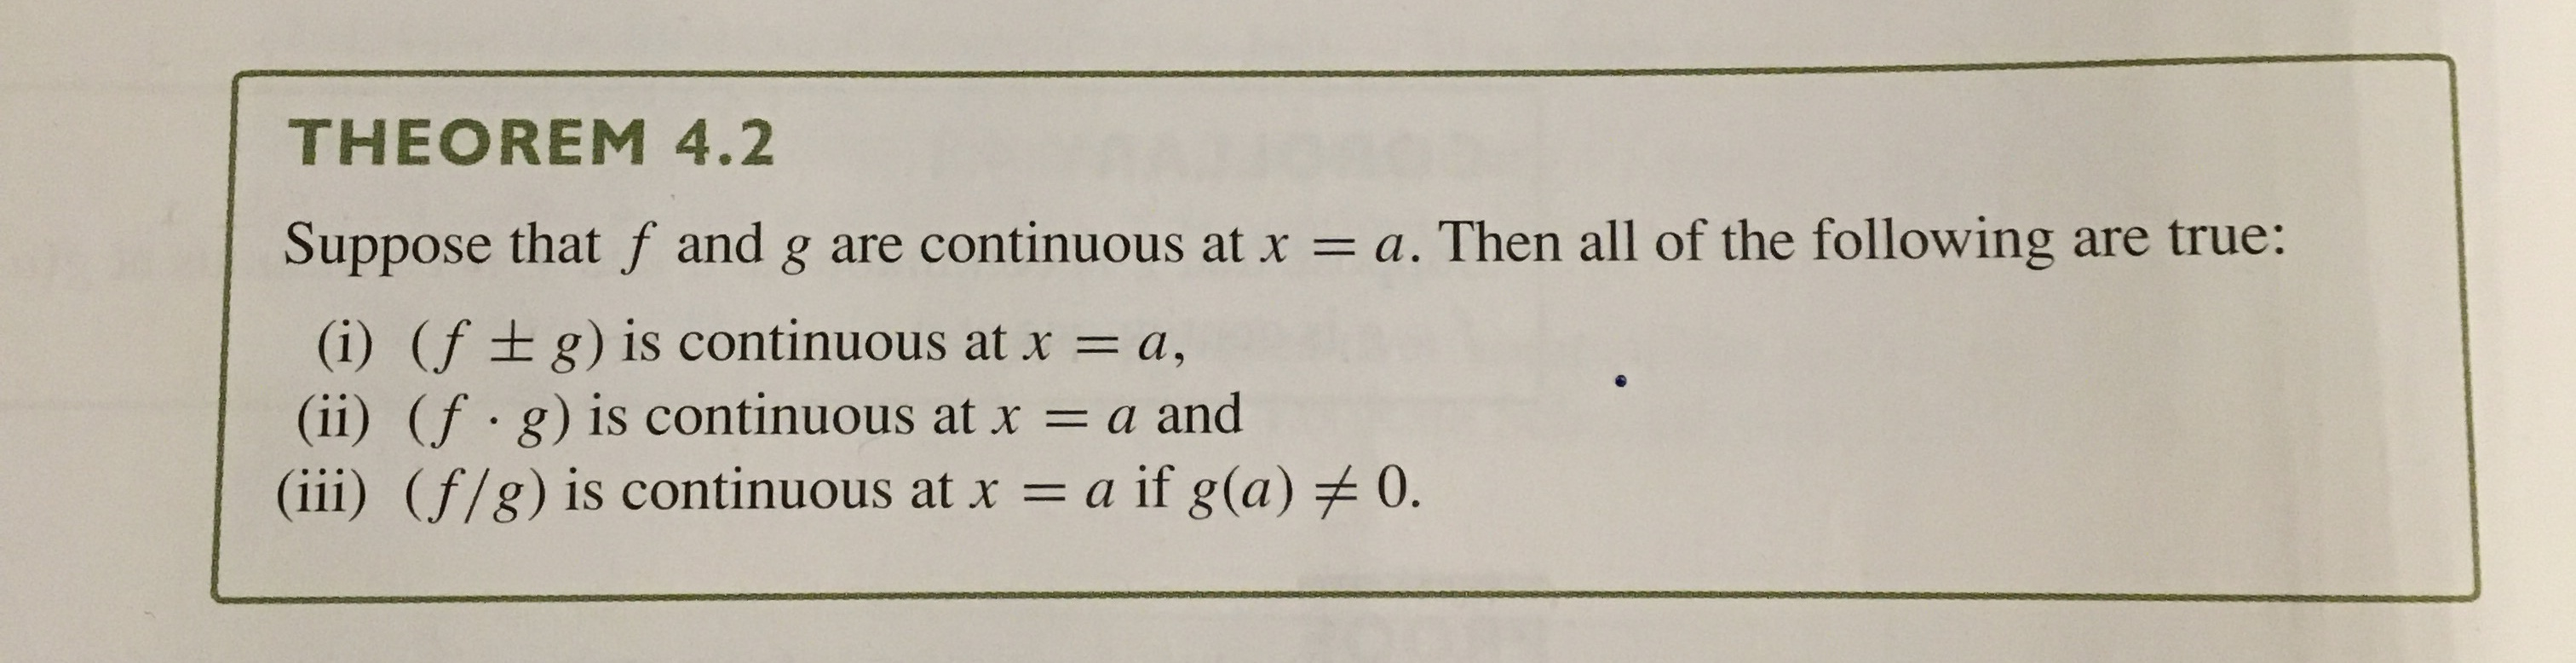
\includegraphics[width=\linewidth]{Pre-Reading/Chapter 1/IMG_0966.JPG}
    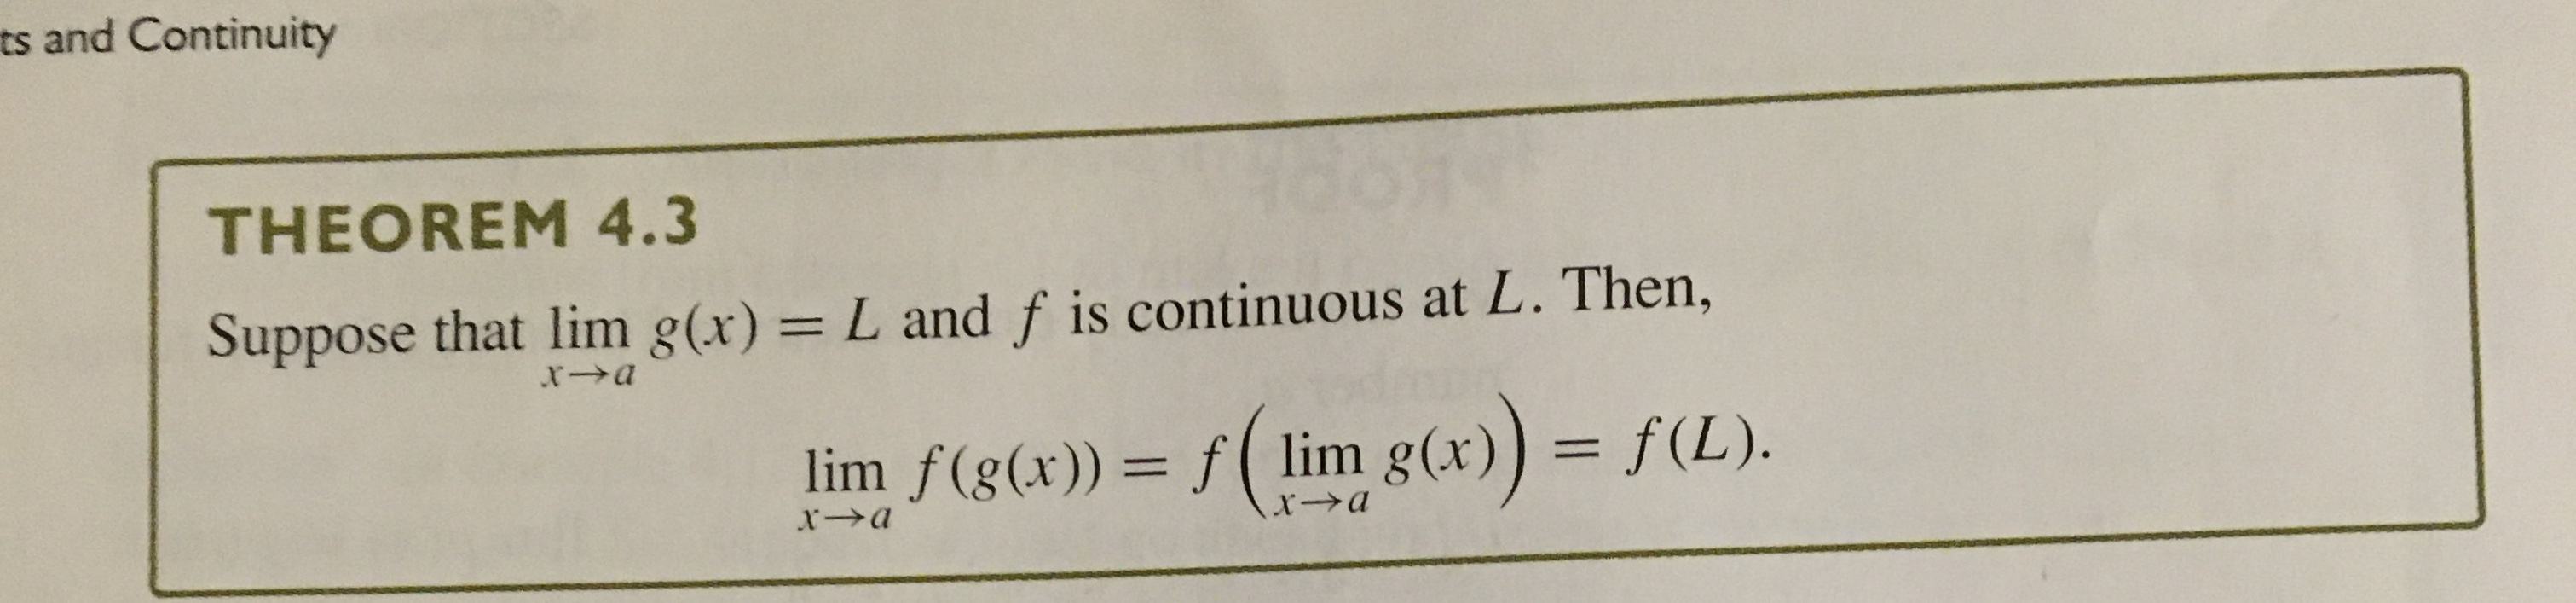
\includegraphics[width=\linewidth]{Pre-Reading/Chapter 1/IMG_0967.JPG}
    
\includegraphics[width=\linewidth]{Pre-Reading/Chapter 1/IMG_0968.JPG}
    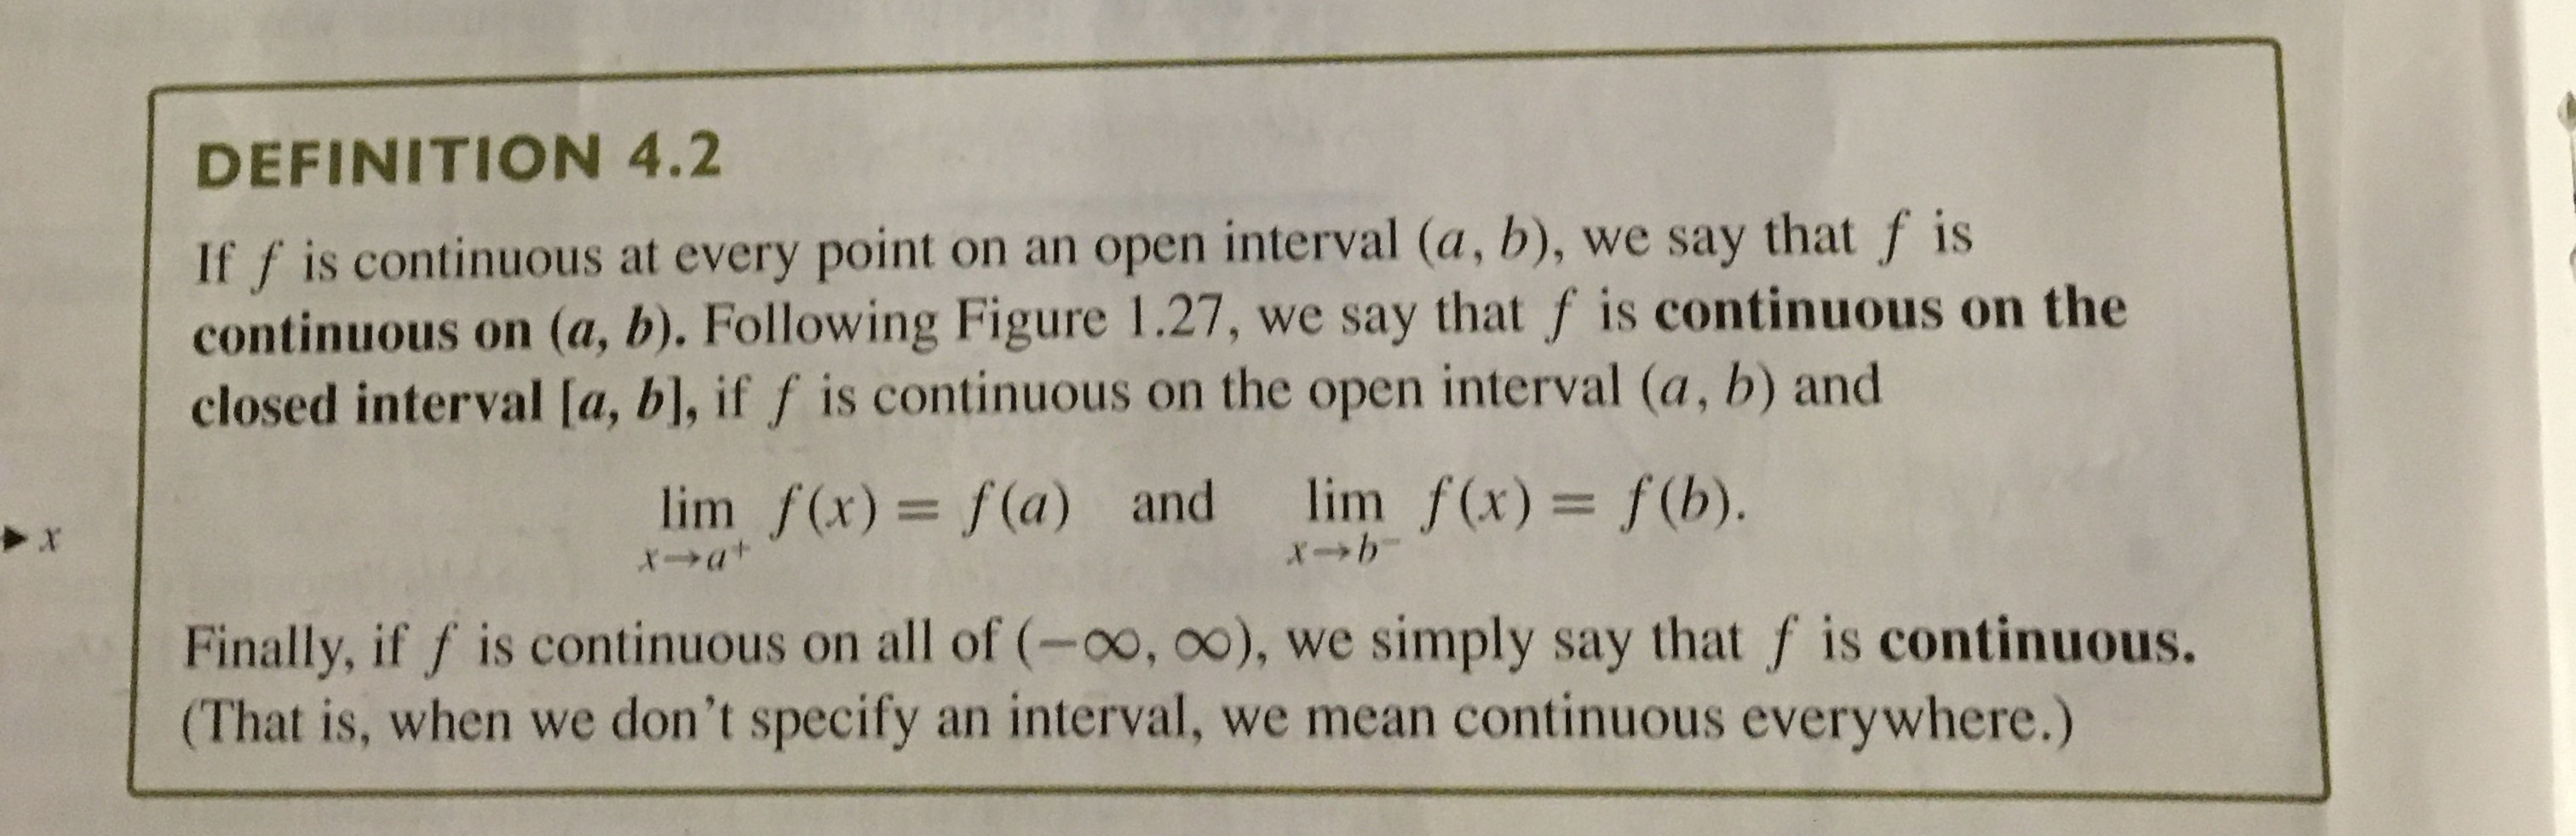
\includegraphics[width=\linewidth]{Pre-Reading/Chapter 1/IMG_0969.JPG}
    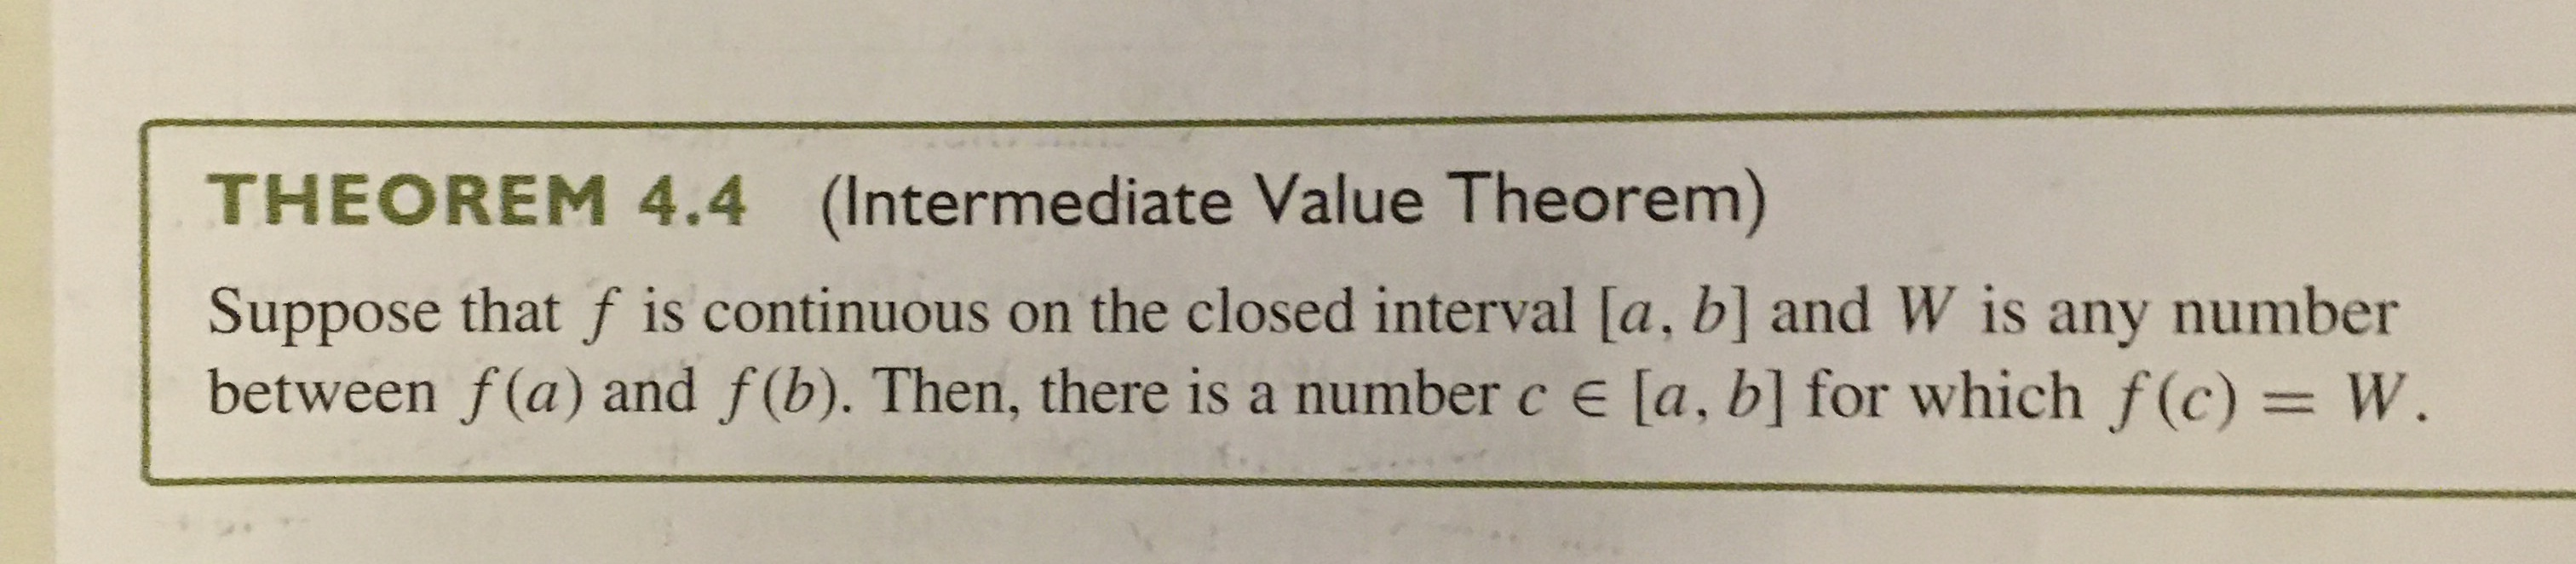
\includegraphics[width=\linewidth]{Pre-Reading/Chapter 1/IMG_0970.JPG}
    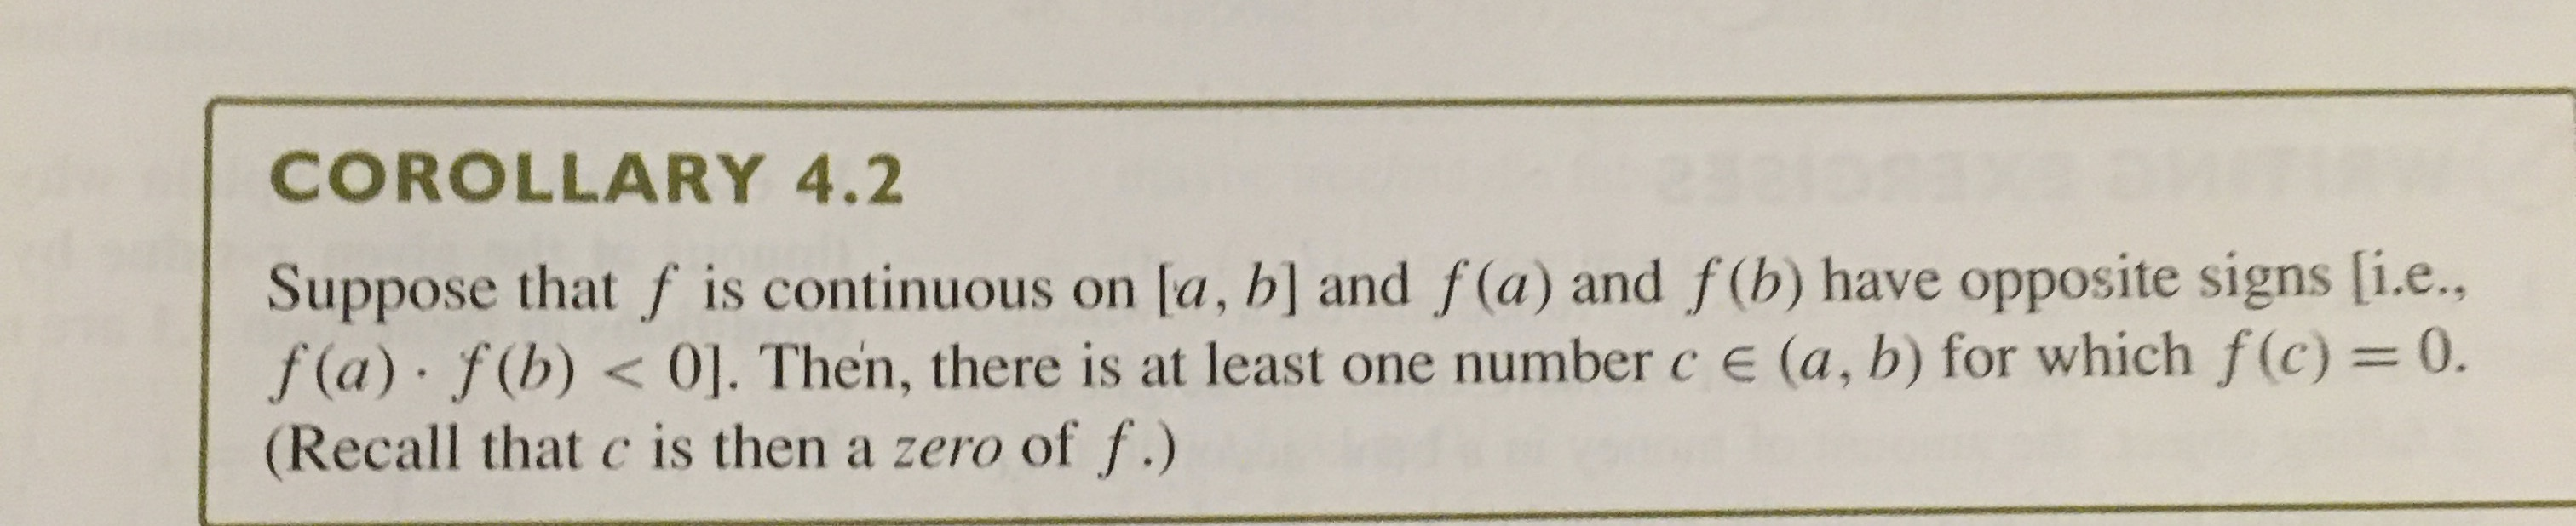
\includegraphics[width=\linewidth]{Pre-Reading/Chapter 1/IMG_0971.JPG}

    \subsection{Limits Involving Infinity: Asymptotes}
    \begin{itemize}
        \item We can express Asymptotes as Limits
        \item Ex: Reciprocal function
    \end{itemize}
    %Insert Diagram Here (1)
    \begin{center}
        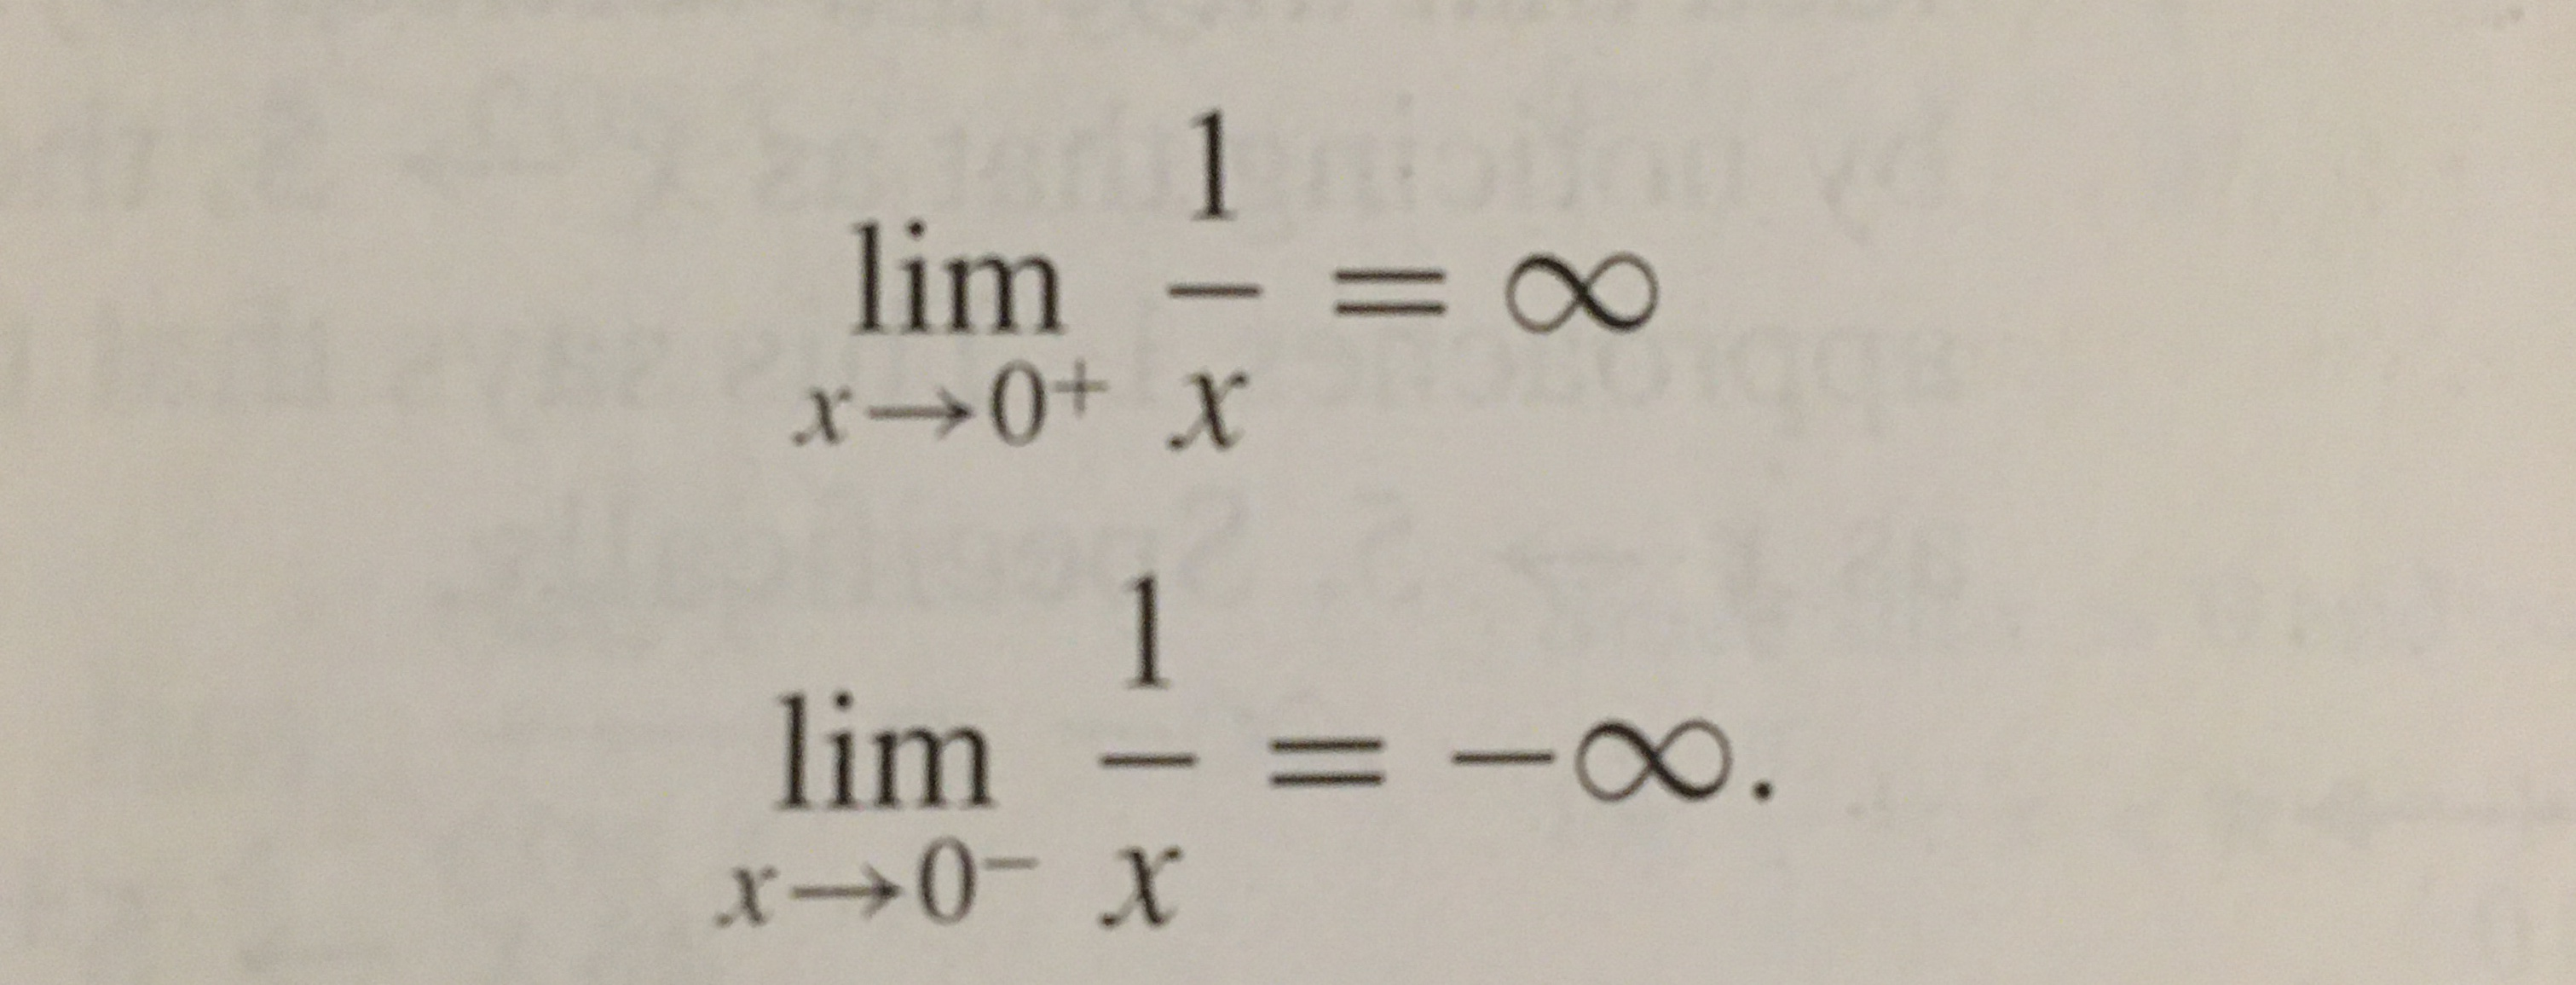
\includegraphics[scale=0.1]{Pre-Reading/Chapter 1/IMG_0972.JPG} 
    \end{center}

\end{document}